\appendix
\section{Appendix}
\subsection{Varying the parameters of the Aliev \& Panfilov model}
\label{app:ap-params}

Here is a quick study presented, which varies the parameters of the phenomenological
Aliev-Panfilov model \eqref{eq:ap_eqs} and examines its behaviour:
tab.~\ref{tab:apparams} gives an overview including a description of the
resulting change and in fig.~\ref{app:apparams} these changes were plotted.

\begin{table}[h]
    \centering
    % {\renewcommand{\arraystretch}{2}%
    \begin{tabular}{C c p{8cm}}
        \toprule
        \text{Name} & Range & Effect \\
        \midrule
        a & \numrange{.1}{.2} &
            \tabitem delay of $V$ and $W$ \\
        & & \tabitem $a=0.2$: both variables are extinguished \\[.6em]
        k & \numrange{4.}{14.} &
            \tabitem scaling strength and slope of $W$ \\
        & & \tabitem the larger $k$, the faster and stronger
            rises $W$ \\[.6em]
        \epsilon_0 & \numrange{1e-5}{1.} &
            \tabitem makes $W$ rise earlier \\
        & & \tabitem maintains the peak's shape \\[.6em]
        \mu_1 & \numrange{.05}{2.} &
        \tabitem makes $W$ rise earlier and steeper \\[.6em]
        \mu_2 & \numrange{.1}{5.} &
        \tabitem delays $W$ and flattens the peak \\[.6em]
        \bottomrule
    \end{tabular}%}
    \caption{Parameter overview}
    \label{tab:apparams}
\end{table}

\begin{figure}[b]
    \centering
    \begin{subfigure}[b]{\textwidth}
        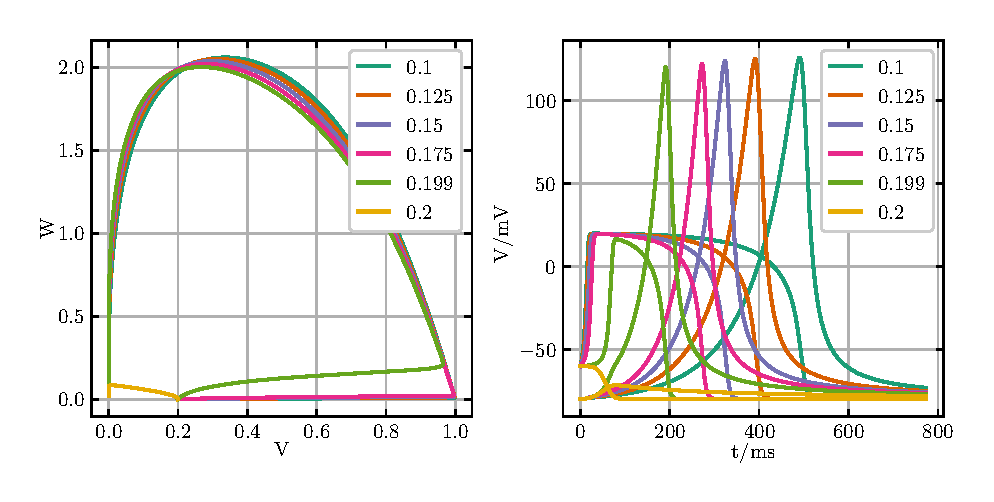
\includegraphics[width=\textwidth]{alpha-params-1}
        \vspace{-2\baselineskip}
        \caption{a}
    \end{subfigure}
    \begin{subfigure}[b]{\textwidth}
        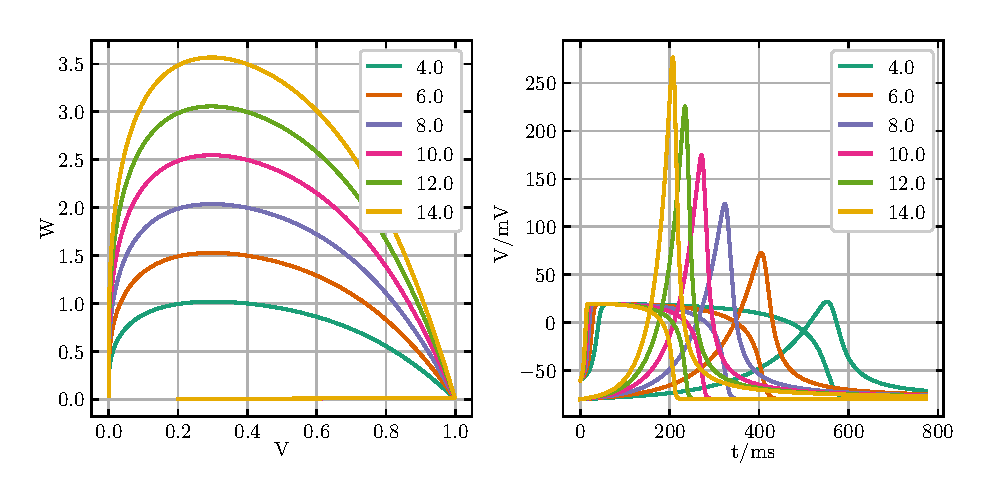
\includegraphics[width=\textwidth]{alpha-params-2}
        \vspace{-2\baselineskip}
        \caption{k}
    \end{subfigure}
    \begin{subfigure}[b]{\textwidth}
        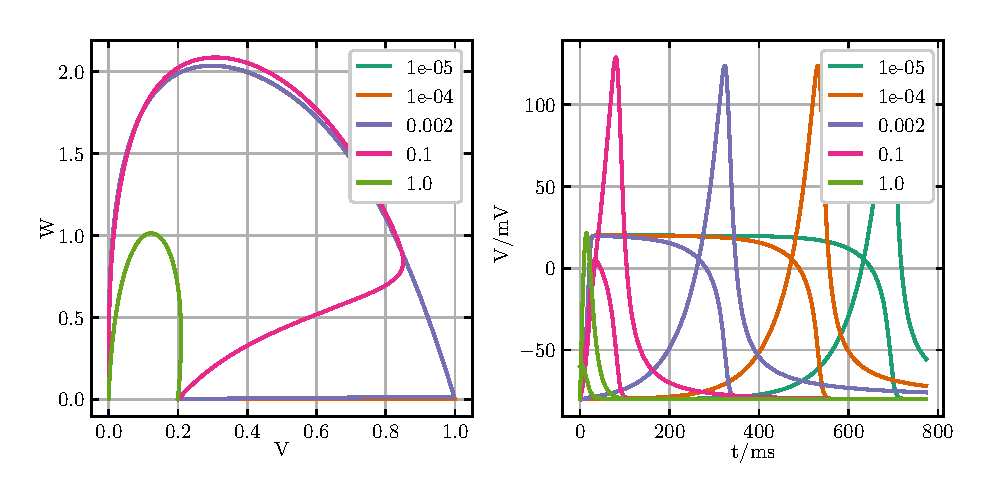
\includegraphics[width=\textwidth]{alpha-params-3}
        \vspace{-2\baselineskip}
        \caption{$\epsilon_0$}
    \end{subfigure}
\end{figure}
\begin{figure}[t]
    \ContinuedFloat
    \centering
    \begin{subfigure}[b]{\textwidth}
        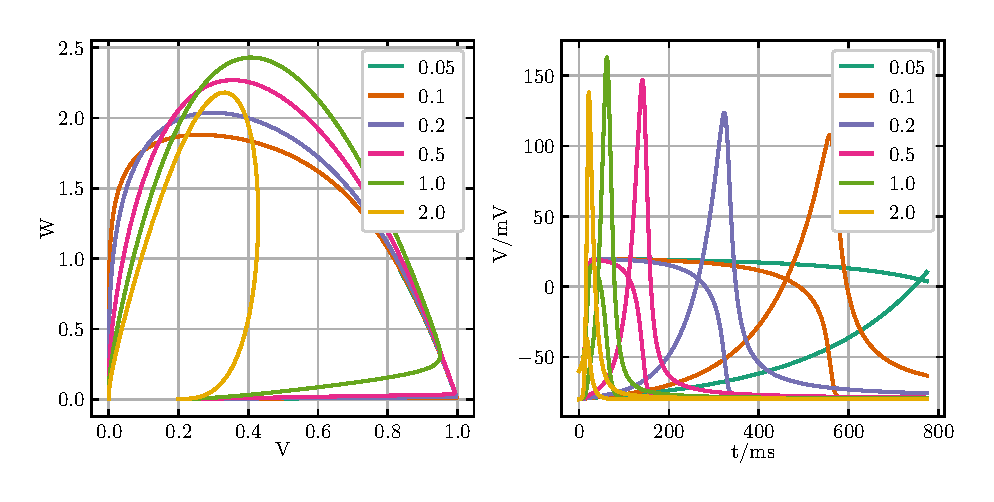
\includegraphics[width=\textwidth]{alpha-params-4}
        \vspace{-2\baselineskip}
        \caption{$\mu_1$}
    \end{subfigure}
    \begin{subfigure}[b]{\textwidth}
        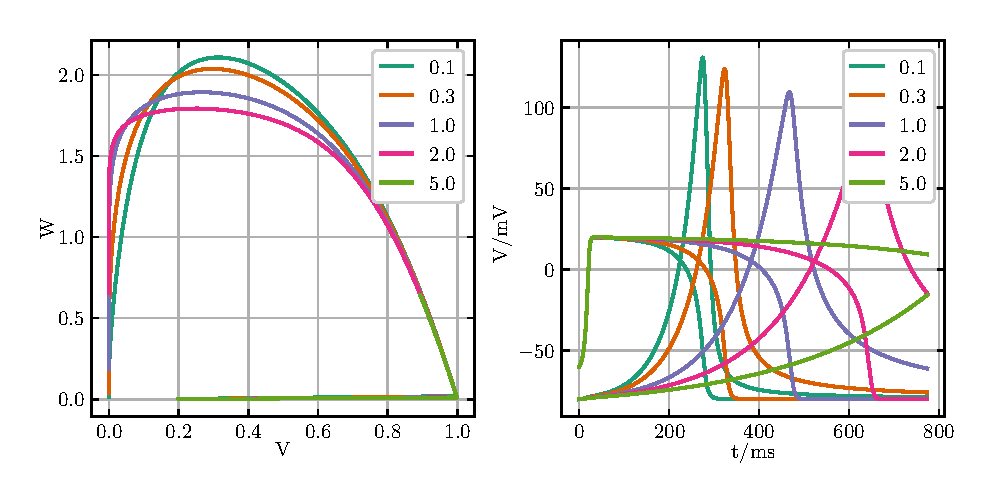
\includegraphics[width=\textwidth]{alpha-params-5}
        \vspace{-2\baselineskip}
        \caption{$\mu_2$}
    \end{subfigure}
    \caption{Plots for varying parameters}
    \label{app:apparams}
\end{figure}


% vim: set ff=unix tw=79 sw=4 ts=4 et ic ai :
